\documentclass[a4paper,twoside]{article}
\usepackage[T1]{fontenc}
\usepackage{graphicx}
\usepackage{amsmath,amssymb,amsthm}
\usepackage{booktabs}
\usepackage{array}
\usepackage{pslatex}
\usepackage{apalike}
\usepackage{algorithm2e}
\usepackage[bottom]{footmisc}
\usepackage{url}
\usepackage[hidelinks]{hyperref}
\usepackage{balance}
\usepackage{SCITEPRESS}
\newcommand{\ind}{\mathbf{1}}
\newcommand{\loss}{\mathcal{L}}
\newcommand{\E}{\mathbb{E}}

% Avoid carrying a hyphenated word fragment across a page boundary.
\brokenpenalty=10000
\newcommand{\draftcredit}{\footnote{Drafting assistance: OpenAI Codex \cite{openai2026codex}. See the AI assistance disclosure.}}

\begin{document}
\title{Supplement to Planning Shared Review for Language Model Workflows with Expiring Intervention Opportunities}
\author{\authorname{Anonymous Companion Material}}
\keywords{Reproducibility, Review Semantics, Paired Evaluation.}
\abstract{This companion documents measured air-handler diagnosis, fallible model review, synthetic scheduling mechanisms and adapted retail transfer. It provides source provenance, whole-day splits, reviewer transition counts, paired capacity sensitivities, queue timelines and reproduction procedures. Measured signals and experimentally imposed labels remain distinct from generated proposals and assumed oversight dynamics. Complete historical maintenance and retail tables retain positive, null and unfavorable findings, including unresolved preparation failures. The main paper contains the formulation and central comparisons needed to assess its claims. This supplement supplies detailed inspection material and is a local research companion, not a claim of an accepted supplementary submission under conference policy.}
\onecolumn\maketitle\normalsize\setcounter{footnote}{0}\vfill

\section{MEASURED HVAC EVIDENCE AND SENSITIVITY}
\noindent The primary measured application uses the collection of \cite{granderson2020data}, specifically Figshare article 11752740, version 3, under its CC0 dedication. Only SZCAV.csv and SZVAV.csv are selected. Source checksums, inventory tables, all day assignments, public summaries and selected one-minute signals are saved with the evidence. The original CSV downloads remain outside Git. The source contains manually imposed faults on one FLEXLAB air handler; labels are experimentally established conditions, while scheduling and weighted consequences are constructed.\draftcredit

\subsection{Source and Information Boundaries}
All 26 recorded days are included, with eight development days and 18 evaluation days. Each contributes three windows, totaling 78 distinct source windows. The initial and revised development collections reuse the same 24 development windows and do not create additional source units. Evaluation has one generation replicate. Source date, filename, fault indicator and imposed-condition description are evaluator-only. Control mode and recording hour are public. Dates are not needed for diagnosis and are excluded to reduce answer-bearing metadata exposure. Public-source pretraining contamination cannot be ruled out.

The three tickets from an experimental day are correlated snapshots of the same equipment under the same imposed condition. They are retrospectively available after the final window closes. Their simultaneous arrival is an assumed backlog condition, not an observed pattern of building fault incidence. A policy changes a recorded diagnosis, not a sensor trajectory. Labels support diagnosis scoring but cannot establish repair efficacy, energy savings or physical harm prevention.

Ten channels retain original Fahrenheit units and fractional controls. Means, minima, maxima and first-to-last changes are deterministic within-window summaries. No evaluation normalization is fit. The conventional classifier standardizes 42 public features, comprising 40 statistics, mode and hour, using development means and standard deviations. Zero-variance dimensions receive scale one. It assigns the closest class centroid by squared Euclidean distance. It is a transparent baseline rather than a tuned state-of-the-art fault detector.

\begin{table*}[t]
\caption{Measured-data evaluation by experimentally annotated component category. Counts are windows, nested within experimental days on one unit. Proposed and reviewed labels are generated. The conventional baseline uses development data only.}
\centering\small
\begin{tabular}{lrrrrr}
\toprule
Condition & Days & Windows & Proposal correct & Review correct & Baseline correct \\
\midrule
normal & 3 & 9 & 1 & 1 & 6 \\
outdoor damper & 4 & 12 & 0 & 0 & 7 \\
heating valve & 6 & 18 & 18 & 12 & 14 \\
cooling valve & 5 & 15 & 0 & 1 & 0 \\
\bottomrule
\end{tabular}
\end{table*}


\subsection{Frozen Conditions and Resource Use}
The declaration fixes six policies, two weight schemes, one or two review slots, service times one/two/three, and three review-benefit conditions. These give 216 paired policy runs per experimental day and 3,888 total. The primary signed-gain rule, secondary risk-only ablation and ideal reference all reuse the same generated proposal/review pair for each window. No policy gets privileged observations. Review output takes effect only at completed service; invalid output preserves the proposal, while abstention is unresolved. Reviews must finish by cutoff equality. No late result cancels an incurred loss.

Development uses 48 initial and 48 revised calls. Evaluation adds 108 calls. All 204 GPU attempts succeed, with no retry, using 125,765 prompt tokens and 9,131 completion tokens. Maximum actual input and output lengths are 745 and 93 tokens, within the existing 2,048-token context and 128-token output allowance. Total measured generation-request time is 174.66 seconds, and the slowest attempt is 1.73 seconds. This measured latency is distinct from assumed review service time. GPU evidence verifies BF16 on the RTX 6000 Ada, the pinned Qwen revision and zero CPU offloading. Server token and call deltas reconcile exactly.

Signed-gain admission declines all primary reviews because fitted gains are nonpositive. That rule misses the one realized potentially helpful model review while avoiding six harmful changes. These are consequences of a sparse development fit, not an oracle identifying harmful evaluation cases. Review-pair diagnostics contain five wrong-category introductions and one harmful abstention. Four further abstentions occur on already wrong proposals. Aggregate error-risk AUROC is 0.5023, Brier score 0.2305, pooled-development Brier 0.2349 and constant-half Brier 0.2500. The prediction ranking is nearly uninformative despite its modest Brier improvement over the constant reference.

\begin{figure*}[t]
\centering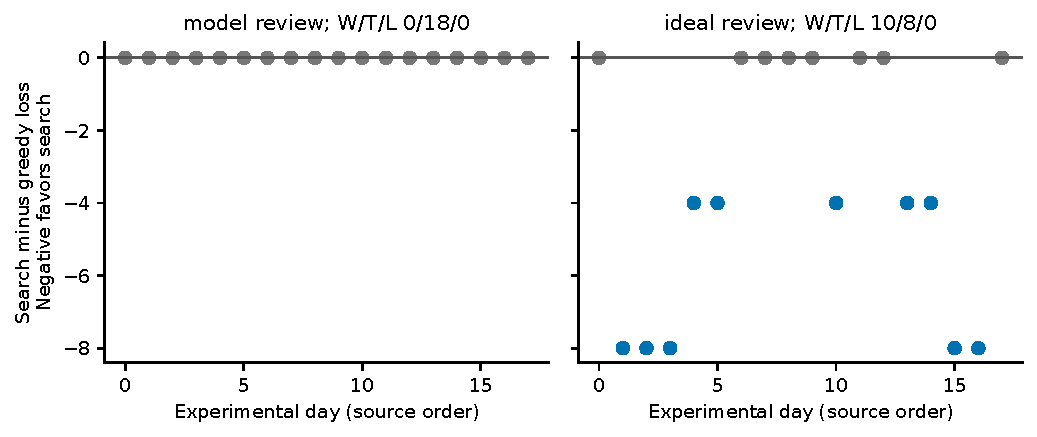
\includegraphics[width=0.98\textwidth]{../artifacts/stage7_empirical/figures/paired_differences.pdf}
\caption{All 18 experimental-day search-minus-greedy differences. Outcomes combine generated diagnoses with annotated correctness and simulated deadlines and weights. The left panel's zero differences follow from a shared admission rule that declines model review. The ideal reference on the right uses corrected labels only at review completion. Days share one physical unit and are not independent buildings.}
\end{figure*}

\begin{figure*}[t]
\centering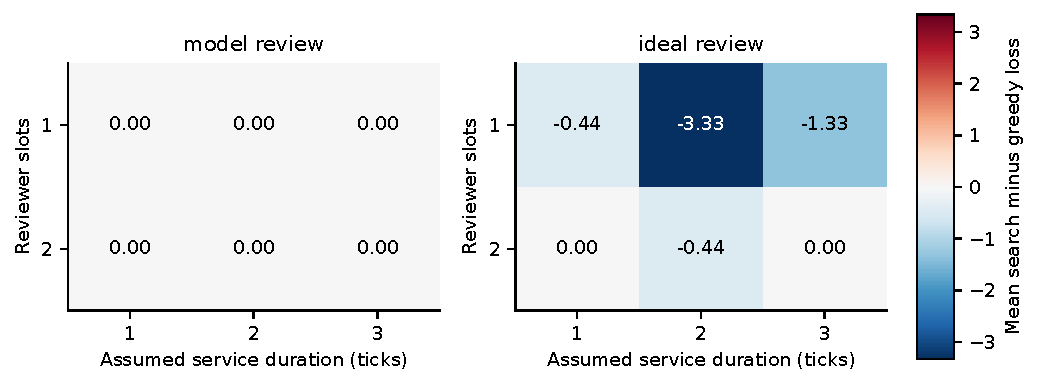
\includegraphics[width=0.98\textwidth]{../artifacts/stage7_empirical/figures/capacity_sensitivity.pdf}
\caption{Prespecified simulated capacity and duration sensitivity on saved measured-data proposals. Cell values are mean search-minus-greedy weighted diagnosis loss. The color scale is centered at zero. Signed model-review admission produces mechanical ties. Ideal review exposes a conditional ordering benefit. These abstract capacities and time units are not measurements of human inspection.}
\end{figure*}

\begin{figure*}[t]
\centering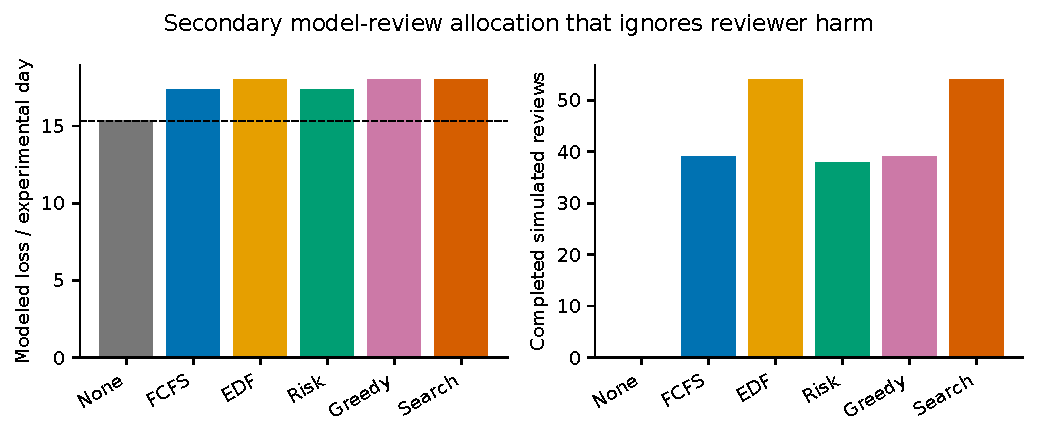
\includegraphics[width=0.98\textwidth]{../artifacts/stage7_empirical/figures/risk_only_secondary.pdf}
\caption{Secondary allocation that substitutes error probability for reviewer effectiveness. The same saved model responses are applied. Loss and review counts are simulated, while correctness is determined by experimental labels. More reviews do not improve diagnosis. Search and greedy tie despite different sequences on 15 of 18 days. The dashed line is no-review loss.}
\end{figure*}

\begin{figure*}[t]
\centering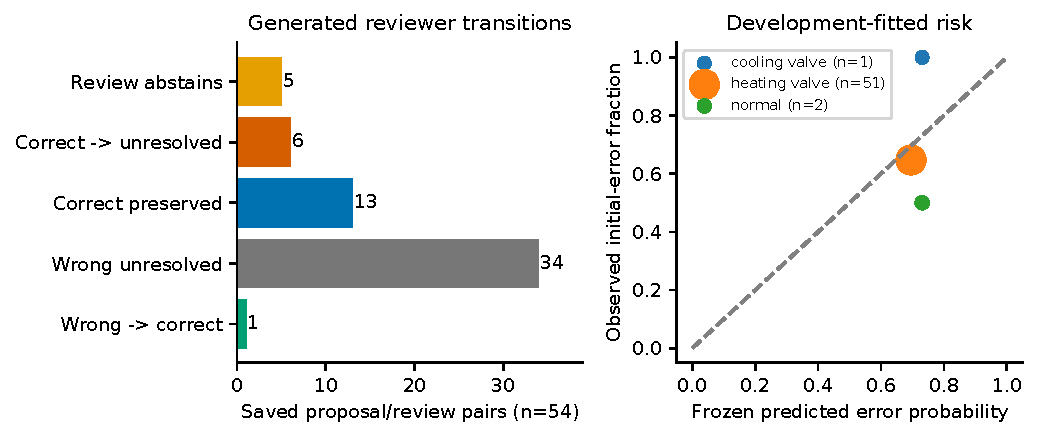
\includegraphics[width=0.98\textwidth]{../artifacts/stage7_empirical/figures/reviewer_risk.pdf}
\caption{Generated reviewer transitions and development-fitted risk on 54 evaluation windows. One correct-to-unresolved transition is an abstention; five change to wrong categories. Abstentions overlap the transition categories. The calibration plot identifies counts for each proposed category, with highly tied risks and small bins. Ground-truth labels are used only in this offline diagnosis, not at dispatch.}
\end{figure*}

\subsection{First-Qualifying Queue Examples}
The rule selects the first numerical source run satisfying each comparison sign, without ranking by effect magnitude. The primary model-review condition has only ties. Its first tie is run01, where no reviews are admitted. The ideal reference has a first benefit at run02, with difference $-8$, and a first tie at run01. Neither has an unfavorable search-minus-greedy case under the declared primary capacity. Absence is reported rather than replacing the rule with a favorable example from another configuration.

\begin{figure*}[t]
\centering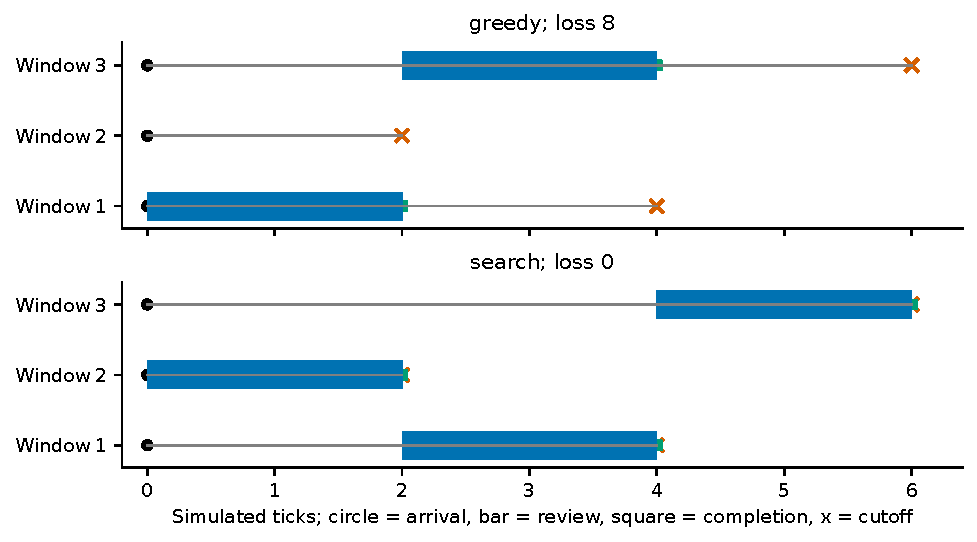
\includegraphics[width=0.88\textwidth]{../artifacts/stage7_empirical/figures/queue_ideal_benefit.pdf}
\caption{First ideal-reference benefit, run02. Both policies receive the same generated diagnoses from measured sensor windows. Bars show simulated review occupancy, squares completion and crosses cutoffs. Search preserves a timely review that greedy misses. Ideal correction is an assumption and this figure is not evidence of successful physical repair.}
\end{figure*}

\begin{figure*}[t]
\centering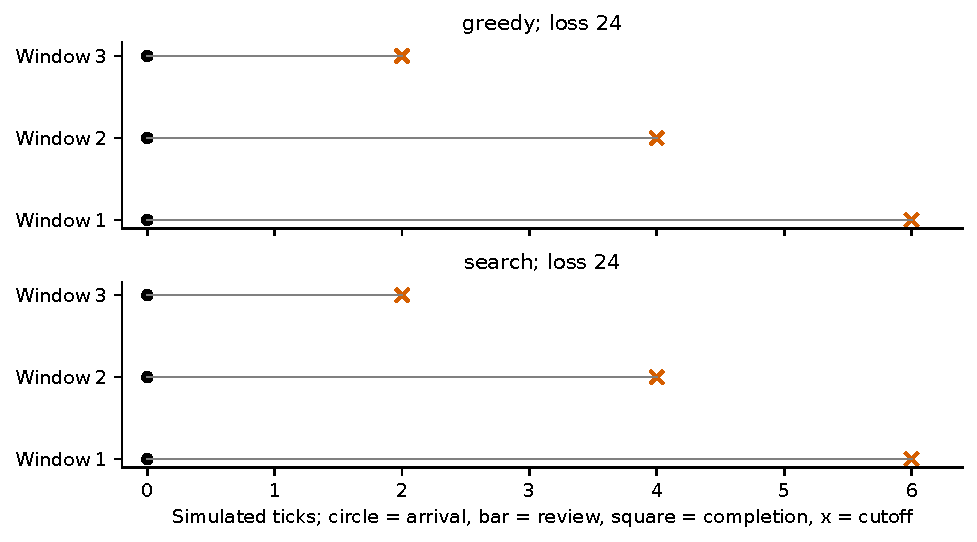
\includegraphics[width=0.88\textwidth]{../artifacts/stage7_empirical/figures/queue_model_tie.pdf}
\caption{First primary-condition tie, run01. All three diagnosis tickets arrive together, but the development-fitted signed gain admits no model reviews. The displayed cutoff events are simulated. Empty review bars reflect the declared decision rule, not missing execution records.}
\end{figure*}

\subsection{Secondary Application Access and Reproduction}
BIRD-Critic-SQLite public records omit reference solutions and hidden tests; the official repository offers them through email contact. No contact was made. BIRD-SQL provides accessible development references and database downloads, but its required database audit and execution study did not fit the remaining original execution deadline. No SQL or optional synthetic fraud result is claimed. This keeps a completed measured primary study separate from unexecuted applications.

The saved-output command is \texttt{bash scripts/replay\_stage7.sh}. It verifies every attempt, frozen input, source summary and policy trace, recomputes tables in a temporary directory, regenerates vector figures, and builds the manuscript and supplement. It does not change the frozen traces or their measured planning latency. Exact GPU regeneration uses the recorded public task files and role prompts, but requires a new explicit authorization and fresh output directory after the historical deadline. Seed reuse alone does not guarantee identical generations.


\section{EVIDENCE ORGANIZATION}
\noindent The evidence package retains immutable declarations, source snapshots, model requests and responses, event traces, estimators and accounting ledgers. Development chronology resides in stage reports rather than the main scientific argument. Original, competition and larger maintenance distributions remain separate. Original retail and the fresh operational follow-up are also separate cohorts.\draftcredit

The completed maintenance evaluation contains 2,752 episodes, with 304 development episodes and 128 separate repeated-request diagnostic generations. Its 48,320 GPU attempts include all development, evaluation and diagnostic calls. The original retail stage contains two preserved pilots, a 72-workflow calibration set and a 288-workflow evaluation. The first pilot staged no transactions; one declared interface revision corrected tool-before-argument serialization and added public progress information. It does not identify the separate causal effects of those two changes. The frozen follow-up leaves this interface unchanged.

\subsection{Maintenance Matrices}
Original scenarios use seeds 10000--10063 and competition uses 11000--11063. Each has six policies and both review durations under frozen agreement risk. The two alternative-risk rules use the first 32 seeds in each workload with greedy and search, while reusing matching frozen rows as the reference. Larger-workload scenarios use 12000--12031, three and six agents, four policies and both durations. The selected objective extension uses 13000--13015 with the declared additional-closure penalties 0, 4 and 8. It is a development-selected objective study, not a universal objective search.

The original distribution and competition matrices contribute 1,536 episodes, alternative-risk rollouts 512, larger workload 512, and the objective extension 192. These are repeated conditions, not 2,752 independent scenarios. The frozen scenario prefixes are not extended based on observed outcomes. All completed traces replay.

\subsection{Observation and Feedback Boundary}
Maintenance model inputs contain released public job information and that agent's own history. Schedulers receive public request records rather than private job objects. Before review completion, neither has definitive fault labels. Reviews finish before same-tick deadline closure, so equality can prevent a terminal penalty. Downtime accumulated before correction remains. Search has no access to the generator's future waves.

Retail preparation has its own agent history and no access to annotated targets. Authentication, account ownership, retrieval and confirmation checks apply before a mutation can be staged. The scheduler then receives only arrived transaction requests and public risk, cost, cutoff and service-time fields. Hidden proposal correctness is consulted by completed perfect review and offline scoring. Other-policy choices logged on the same public state are diagnostics and do not alter the executed policy.

\section{SYNTHETIC MECHANISM DETAILS}
\noindent The maintenance environment exposes binary ventilation faults through two independent noisy clues. Faults have equal prior probability, with clue accuracies 0.8 and 0.6. An agent chooses a filter replacement or sensor reset from a public manual. Two fresh model samples are drawn per job. The first action executes; the second supplies agreement information. Review may correct the executed action and provide definitive feedback for later jobs.\draftcredit

An initially wrong action incurs downtime rate $c_i$ until correction or deadline, plus terminal incorrect-closure penalty $K_i$. A timely correction at $T$ prevents
\begin{equation}
 G_i(T)=\ind[T\leq d_i]\{c_i(d_i-T)+K_i\}.
 \label{eq:maintenance}
\end{equation}
The original workload uses three agents, two jobs each and a 12-tick horizon. Releases occur at wave bases 0 and 6 with zero-or-one jitter. Relative windows are drawn from 1, 2 and 5, downtime rates from 0, 1 and 3, and terminal penalties from 0 and 8.

A constructed competition workload releases all three jobs together at 0 and 6. Each wave independently permutes windows 2, 4 and 5 and penalties 4, 8 and 12, with zero downtime. It was motivated by limited competition in earlier development, then evaluated on new frozen scenarios. A larger workload has three or six agents, three jobs each, a 24-tick horizon and waves at 0, 8 and 16 with independent zero-or-one jitter. Windows are 2, 4 and 6, downtime rates 0, 1 and 3, and penalties 0, 4, 8 and 12. Stable per-agent streams pair the first three agents across team sizes. Public assignments are independent of hidden faults.

\subsection{Risk and Frozen Evaluation}
The primary risk estimate is an agreement-bin estimator fit on an earlier development set. Laplace smoothing gives $(e+1)/(n+2)$ for $e$ errors among $n$ jobs; bins with fewer than ten examples use pooled calibration risk. Initial first-action labels are included regardless of review selection. The frozen values are $13/89$ for agreement and pooled $18/98$ for sparse disagreement.

Alternative estimates use pooled risk or a public analytical reference with knowledge of the synthetic observation model. Following agreeing clues has error probability $1/7$; following the stronger disagreeing clue has error probability $3/11$. Choosing the opposite action gives the complementary probability. The reference does not inspect the realized fault. Both samples are retained in every condition. Prediction rescoring uses saved outputs; policy comparisons under alternative risk use actual new trajectories.

The frozen evaluation contains 2,752 episodes. Original and competition workloads each use 64 scenarios and six policies at one- and two-tick reviews. Alternative-risk comparisons use the first 32 scenarios of each workload for greedy and search. Larger-workload comparisons use 32 scenarios with four policies across both team sizes and capacities. A separately declared objective study uses 16 scenarios. The development and evaluation partitions remain separate.

\subsection{Results and Boundary Conditions}
Table~\ref{tab:maintenance} reports central search--greedy contrasts. At two ticks, search gains in constructed competition but has little measured advantage in the original workload. It wins, ties and loses against greedy on 15, 42 and 7 competition scenarios, versus 3, 59 and 2 original scenarios. Search versus EDF in two-tick competition is $-2.5625$ points, with interval [$-4.0000,-1.3125$]. At one tick, search and EDF both attain zero competition loss despite different review sequences on 62 of 64 scenarios.

\begin{table*}[t]
\caption{Frozen maintenance results. Differences are search minus greedy mean loss with 95\% paired scenario-bootstrap intervals. Workload distributions are analyzed separately.}
\label{tab:maintenance}\centering\small
\begin{tabular}{llrrrrl}
\toprule
Workload & Agents / scenarios & Review ticks & Search & Greedy & EDF & Paired difference \\
\midrule
Original & 3 / 64 & 2 & 7.328 & 7.422 & 7.656 & $-0.094\;[-0.563,\;0.344]$ \\
Competition & 3 / 64 & 2 & 1.688 & 3.000 & 4.250 & $-1.313\;[-2.250,-0.438]$ \\
Competition & 3 / 64 & 1 & 0.000 & 0.375 & 0.000 & $-0.375\;[-0.688,-0.125]$ \\
Larger & 6 / 32 & 1 & 16.188 & 22.375 & 23.688 & $-6.188\;[-9.376,-3.281]$ \\
Larger & 6 / 32 & 2 & 36.563 & 36.781 & 46.000 & $-0.219\;[-2.313,\;1.969]$ \\
\bottomrule
\end{tabular}
\end{table*}

The larger workload gives a stronger one-tick planning benefit and a small, uncertain two-tick difference. Reduced capacity does not monotonically increase the value of planning. Some requests are already infeasible when the reviewer becomes free. In the original two-tick search runs, only 32 of 156 dispatches have multiple eligible requests, whereas competition has 224 of 256. Such public contention is a prerequisite for many sequencing effects, but it does not guarantee competing actual errors.

Risk calibration and allocation utility diverge. The frozen estimator predicts roughly 0.15 error while observed errors reach about 0.25--0.32. On two-tick search trajectories, analytical risk improves Brier score from 0.213 to 0.157 in the original workload and from 0.200 to 0.164 in competition. Yet fresh matched-prefix alternative-risk rollouts yield no consistent allocation gain. Better probability scores alone do not establish better counterfactual policy performance.

Weighted cost also differs from task correctness. In the six-agent one-tick workload, search has lower loss than EDF but more incorrect closures. Adding a declared penalty $\lambda$ per incorrect closure to the search objective changes both intervention benefit and eligibility. With $\lambda=8$ rather than zero, original cost increases by 1.75 points [$0.188,3.438$], while incorrect closures decrease by 0.75 [$0.375,1.125$] per scenario. The common augmented objective $\loss+8U$ improves by 4.25 points, where $U$ counts incorrect closures. At two ticks this improvement weakens and the augmented objective is slightly worse. This is a tradeoff between objectives, not a universally superior policy.



\section{RETAIL SOURCE AND SEMANTICS}
\noindent The source is the MIT-licensed retail component of $\tau$-bench \cite{yao2024tau}, pinned at revision
\begin{quote}\small\ttfamily
59a200c6d575d595120f1cb70fea53cef0632f6b
\end{quote}
The selected substrate retains all orders for each isolated account and the full product catalog. Tool functions are unmodified. The original package's hosted user simulator is not imported. The adapter reproduces its recursive final-database hash semantics and verifies target mutations on isolated state.\draftcredit

The supported mutation tools are cancellation, pending-order item modification, delivered-order item return and delivered-order item exchange. Account lookup, account retrieval, order retrieval and product retrieval remain genuine tool steps. Item-modification and exchange calls require the full desired list, compatible available variants and valid payment. A wrong but available variant can pass these checks and fail the recorded user intent. Review therefore addresses a different error class from an invalid tool call.

The customer script repeats only the task's operational information. It confirms the proposal that the agent displays, without independently checking product identifiers against hidden targets. This is not an oracle user. The source audit checks intent-to-annotation consistency without model outputs, including order identity, cancellation reason, refund/payment destination, old/new options, unique available target variants, return names and multiplicities. Broad source templates remain shared across partitions.

\subsection{Operational Assumptions}
The following distinctions guide interpretation.
\begin{itemize}
\item A staged mutation is a proposed database operation. Posting it is a committed application transition. Physical delivery, receipt and payment settlement are not simulated.
\item A review cutoff is our constructed latest completion time for preventing the posting consequence. It is not a measured retailer deadline. The backend does not advance a pending order to shipped merely because a tick passes.
\item Corrective review assumes permission to restore the complete recorded intent without renewed customer confirmation. Restricted review removes that power and retains perfect detection only.
\item Blocking a wrong transaction prevents its processing consequence but leaves four points of unresolved service loss. It is neither a completed task nor a successful correction.
\item Complexity time depends on the proposed public item list. If an agent omits an item, the proxy may make that proposal appear simpler. This is retained rather than repaired using hidden targets.
\item Exact database equality may penalize a reason or payment-field difference more strictly than a domain expert's operational equivalence judgment. Such judgments were not collected.
\end{itemize}

Shopify's documented editing, cancellation and return-processing interfaces support the distinction between request, approval and later processing \cite{shopify2026editing,shopify2026cancel,shopify2026returns}. They do not establish the simulation's numerical weights, perfect detection or service times. The source-based methodological review is not independent human expert validation.

\subsection{Risk Estimator}
Calibration includes all 64 successfully staged proposals from 72 development workflows, with labels taken before correction. No reviewed-only label filter is applied. Let a bin have $e$ initial errors among $n$ proposals. Its estimate is $(e+1)/(n+2)$ if $n\geq 10$, otherwise the pooled calibration estimate. The public feature is family plus an uncertainty flag for non-high reported confidence or a previous automatic rejection.

\begin{table}[t]
\caption{Frozen application calibration. All staged examples have the uncertainty flag. Unflagged bins have no examples and use pooled fallback.}
\centering\small
\begin{tabular}{lrrr}
\toprule
Family & Examples & Errors & Risk \\
\midrule
Cancellation & 23 & 0 & 0.0400 \\
Modification & 22 & 6 & 0.2917 \\
Return/exchange & 19 & 9 & 0.4762 \\
Pooled & 64 & 15 & 0.2424 \\
\bottomrule
\end{tabular}
\end{table}

The frozen estimator hash is
\begin{quote}\small\ttfamily
5734f6babfbd33655a76595f001251bd591\\
4d94dde0c0e3401af3fc4a762a581
\end{quote}
No follow-up labels refit it. Prediction diagnostics condition on staging and are identical across scheduling conditions because preparations are shared. Unstaged failures remain in task and loss reporting.

\section{FRESH FOLLOW-UP PROVENANCE}
\noindent The source-pool audit examines all 635 pinned train, dev and test records. It finds 54 customer accounts appearing in multiple splits. Exclusion operates on account identity across splits, not just record IDs. All 120 Stage 5 accounts are excluded, including development and pilot records. Remaining eligible accounts number 10 for modification, 26 for cancellation and 69 for returns/exchanges before cross-family reservation. The 16-bundle target is therefore infeasible. The frozen fallback selects eight bundles from 24 globally unique training accounts. The source split does not establish absence from model training.\draftcredit

Source order is train, dev, test, then ascending index. Modification is reserved first, followed by cancellation and returns/exchanges, with account deduplication throughout. No model outcome influences selection. Three generation replicates use identical case composition and public slot assignments. Scenario seeds 62000--62007 permute arrivals, windows, weights and agent-family order. Generation seeds hash the partition, bundle, case, replicate, step and retry, independently of policy or operational variant.

\begin{table*}[t]
\caption{Fresh bundle composition. Each row is reused across three generation replicates. Values are case ID, arrival, cutoff and processing weight in agent order.}
\centering\small
\begin{tabular}{llll}
\toprule
Bundle & Agent 0 & Agent 1 & Agent 2 \\
\midrule
stage6\_00 & train:313 / 0 / 2 / 8 & train:421 / 0 / 4 / 12 & train:153 / 1 / 6 / 4 \\
stage6\_01 & train:158 / 0 / 2 / 8 & train:320 / 1 / 5 / 12 & train:436 / 0 / 5 / 4 \\
stage6\_02 & train:437 / 1 / 5 / 8 & train:162 / 0 / 2 / 12 & train:323 / 0 / 5 / 4 \\
stage6\_03 & train:167 / 0 / 2 / 4 & train:324 / 1 / 6 / 12 & train:439 / 0 / 4 / 8 \\
stage6\_04 & train:169 / 0 / 4 / 4 & train:338 / 0 / 2 / 8 & train:450 / 1 / 6 / 12 \\
stage6\_05 & train:174 / 0 / 5 / 12 & train:455 / 1 / 5 / 8 & train:341 / 0 / 2 / 4 \\
stage6\_06 & train:466 / 0 / 5 / 4 & train:177 / 1 / 5 / 8 & train:356 / 0 / 2 / 12 \\
stage6\_07 & train:357 / 0 / 2 / 4 & train:482 / 1 / 5 / 12 & train:178 / 0 / 5 / 8 \\
\bottomrule
\end{tabular}
\end{table*}


The full frozen follow-up is 72 workflow attempts and 864 policy episodes. Its maximum preparation cost is 1,008 ordinary calls or 2,016 attempts with one retry per call. The stage-wide ceiling is 6,000 attempts. Model settings, source hashes, estimator, conditions, comparisons and failure handling were committed before the first fresh call. No difficult case is replaced.

\section{OPERATIONAL ROBUSTNESS STUDY}
\noindent A source-based methodological review identified corrective authority, confirmation, family-specific processing stages, review complexity and consequence valuation as unresolved assumptions. It was not independent human expert validation. We froze two one-factor changes, retaining the original condition at both base capacities, the same six policies and the frozen application estimator.\draftcredit

\subsection{Authority and Complexity Changes}
Under restricted authority, a completed review perfectly detects whether the staged proposal is wrong. A correct proposal is approved unchanged. A wrong proposal is blocked, leaving the account unchanged and the service unresolved. It is removed from the queue and cannot post later. Blocking counts neither as task completion nor correction. The preventable loss is therefore
\begin{equation}
 G_i^{\mathrm{block}}(T)=\ind[T\leq d_i]W_i.
 \label{eq:block}
\end{equation}
The missing service benefit is substantive. Since $W_i$ varies, replacing $4+W_i$ by $W_i$ is not a uniform rescaling and can change risk-weighted rankings. Perfect detection remains idealized, and labels are still unavailable before completed review.

The separate complexity condition retains full correction authority and uses
\begin{equation}
 s_i=s+\ind[\text{proposed item-list length}\geq 2],
 \label{eq:complexity}
\end{equation}
where $s$ is one or two ticks. This public proxy captures an additional item-checking burden without fitting review times. A mistaken omission may reduce the apparent complexity, which is retained as a limitation. Arrivals, cutoffs, consequence weights, preparation and risk remain unchanged. We do not evaluate an authority-by-complexity factorial design.

Two outcomes follow mathematically. No-review loss is invariant across variants. Under perfect blocking, every policy's correct-task count equals the initially correct staged count, since neither a wrong nor an unstaged request can be completed by blocking. These invariances are semantic checks rather than empirical discoveries.

\subsection{Fresh Source Cases and Analysis}
We audit all 500 train, 20 dev and 115 test records at the pinned revision, excluding all 120 Stage 5 accounts across source splits. Eligibility retains the original explicit-instruction, supported single-transaction criteria and source-intent consistency checks. Only ten unused eligible modification accounts remain, so a 16-bundle design is infeasible. The declared fallback selects eight globally disjoint bundles from 24 training cases, reserving modification first and then cancellation and returns/exchanges in source order. The source pool is not filtered using model outcomes or expected scheduling gains.

Three fresh replicates yield 72 workflow attempts. The same preparations feed six policies, two base durations and three operational variants, giving 864 policy episodes without repeated GPU calls for scheduling. The primary comparison is search minus greedy under restricted authority at base duration two. We average replicates within each of the eight bundles and use 2,000 common-index bootstrap draws with seed 20260916. Individual bundle differences accompany the interval. The same variants applied to the earlier 32 bundles are explicitly post hoc saved-data sensitivity, analyzed separately and never pooled with the fresh cases.

\subsection{Fresh Results}

All 72 workflow attempts are retained. Fifty-one stage a transaction, 39 are initially correct and 12 stage a wrong valid transaction. Twenty-one do not stage, comprising 18 step-limit failures and three finishes without a transaction. All 675 GPU generations succeed, with no retry. Table~\ref{tab:fresh} gives every policy and condition.

The primary restricted-authority difference is $+1.667$ loss points for search minus greedy, with a 95\% paired interval of $[0.000,4.667]$. Search wins on zero bundles, ties on six and loses on two. The eight bundle-mean differences in numerical order are $0,0,0,0,0,0,1.333,12.000$. The wide interval reflects a small, sparse sample and does not establish equivalence or a general population disadvantage.

Search blocks eight wrong transactions versus greedy's twelve and lets four wrong transactions post. Both complete 39 of 72 tasks because blocking cannot complete a wrong or unstaged request. Search performs 44 reviews versus 42, consuming 88 versus 84 ticks. Its loss is 172 points versus 132, or 7.167 versus 5.500 per three-case run. EDF has mean loss 7.000. The secondary search--EDF difference is $+0.167\;[0.000,0.500]$, with seven bundle ties and one loss.

\begin{table*}[t]

\caption{Fresh follow-up mean loss. Each cell represents 24 runs on eight source bundles. C and X are correct-task totals at base duration two for correction and complexity time, with denominator 72. Approve/block completes 39 tasks under every policy. No-review inputs are identical across conditions.}

\label{tab:fresh}\centering\small

\begin{tabular}{lrrrrrrrr}

\toprule

& \multicolumn{2}{c}{Correction} & \multicolumn{2}{c}{Approve/block} & \multicolumn{2}{c}{Complexity time} & \multicolumn{2}{c}{Correct} \\ Policy & 1 tick & 2 ticks & 1 tick & 2 ticks & 1 tick & 2 ticks & C & X \\

\midrule

No review & 9.833 & 9.833 & 9.833 & 9.833 & 9.833 & 9.833 & 39 & 39 \\

FCFS & 3.500 & 5.500 & 5.500 & 7.000 & 3.500 & 5.833 & 48 & 47 \\

EDF & 3.500 & 5.500 & 5.500 & 7.000 & 3.500 & 5.833 & 48 & 47 \\

Uncertainty & 3.500 & 3.500 & 5.500 & 5.500 & 3.500 & 3.833 & 51 & 50 \\

Greedy & 3.500 & 3.500 & 5.500 & 5.500 & 3.500 & 3.833 & 51 & 50 \\

Search & 3.500 & 5.833 & 5.500 & 7.167 & 3.500 & 6.167 & 47 & 46 \\

\bottomrule

\end{tabular}

\end{table*}



At one tick, every review policy prevents every staged error in all three variants. Correction and complexity time reach the 21-unstaged-failure floor of 84 loss points. Blocking instead retains unresolved service loss for all 33 initially unsuccessful requests, totaling 132 points. These distinct floors follow from corrective authority, not from a better scheduling rule.

At two ticks, full correction gives search minus greedy $+2.333\;[0.000,6.333]$. The complexity variant has the same paired difference while increasing both policies' loss by one third of a point. Only six staged proposals from four cases trigger the added tick, including two initially wrong proposals. This limited exposure bounds what the complexity null contrast establishes.

Approve/block leaves every fresh review sequence unchanged relative to correction. Its smaller search--greedy loss difference is therefore explained by the changed preventable consequence, not an observed improvement in allocation. The benefit functions can produce different rankings in arithmetic cases, but do not do so in these fresh trajectories.

\begin{figure*}[t]

\centering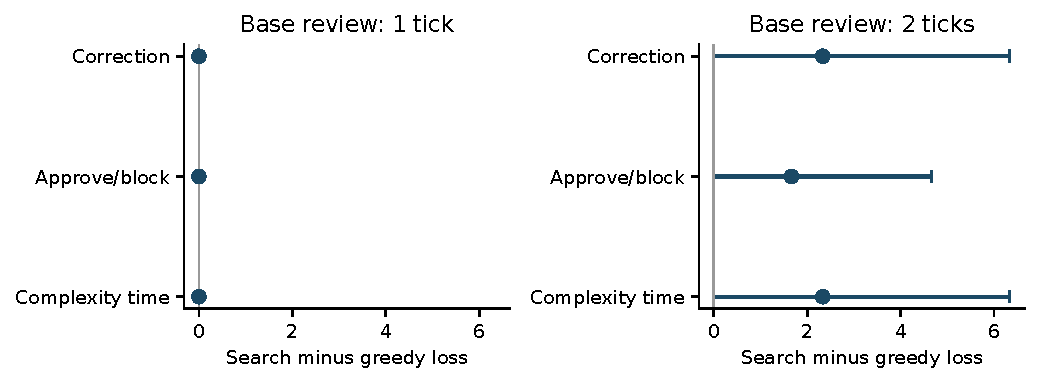
\includegraphics[width=0.98\textwidth]{../artifacts/stage6_robustness/analysis/fresh/figures/paired_loss.pdf}

\caption{Fresh operational sensitivity. Points are search minus greedy mean loss; bars are 95\% paired bundle-bootstrap intervals. Only approve/block at base duration two is primary. Degenerate one-tick intervals describe ties in this sample, not population equivalence.}

\label{fig:robustness}\end{figure*}

\subsection{Scheduling Mechanism and Error Ranking}

Search and greedy review sequences differ in six of 24 fresh runs at base duration two, versus one search--EDF difference. On search's states, 19 dispatches have multiple eligible requests and six have different greedy/search heads. These are repeated states for descriptive analysis, not additional independent observations.

The first unfavorable example is bundle 06, replicate 2. At tick zero, search reviews a correct cancellation with cutoff two, planning to preserve both currently available opportunities. Greedy instead blocks the wrong modification by tick two. A correct exchange arrives at tick one. When search becomes free, its frozen estimate prioritizes that exchange, and the modification posts at tick five. Search loss is eight versus greedy's four. The primary example rule finds no fresh search benefit. The first tie contains a blocked incomplete return and an unstaged modification, giving equal loss eight.

The frozen estimator's aggregate Brier score is 0.17144, versus 0.17998 for its pooled estimate; AUROC is 0.6581. Yet modification has eight errors among 13 staged proposals, versus four among 18 returns/exchanges, while predicted risks rank those families in the opposite order. All 20 staged cancellations are correct. This retrospective evidence helps explain the unfavorable trace without granting labels to the scheduler or refitting on evaluation data. Eight source cases produce different proposals across the three replicates, and four have mixed initial correctness.

\subsection{Saved-Preparation Sensitivity}

The separate post hoc analysis replays all 1,152 original reference traces exactly and adds the declared variants on the same 288 preparations. At base duration two, restricted-authority search minus greedy is $+0.125\;[-0.167,0.500]$, with one win, 29 ties and two losses. Complexity time gives $+0.500\;[-0.083,1.250]$, with one win, 28 ties and three losses. These results do not replace the original $+0.250$ primary comparison. Blocking changes search's actual sequence in only two of 96 runs relative to correction. The first saved-data benefit remains available as a trace alongside the fresh null and unfavorable examples.




\section{PAIRED ANALYSIS DETAILS}
\noindent For each source bundle, the three generation replicates are averaged before comparing policies. Bootstrap draws resample entire bundles, with all conditions kept together. The fresh sample therefore has eight independent bundle units. The post hoc sensitivity uses 32 earlier bundles and is not pooled with it. Fixed seed 20260916 generates 2,000 common-index resamples for the follow-up analyses.\draftcredit

The original Stage 5 primary interval remains [$-0.3333,1.0000$] with its original analysis seed. Recomputing the same reference rows with the newly declared common bootstrap seed gives a slightly different upper endpoint, 0.9167. This finite Monte Carlo difference does not reflect changed outcomes. Both records are preserved.

A reporting-direction defect in secondary completion rows was detected and repaired. The initial code labeled a negative completion difference as a win because it inherited the loss convention. The corrected labels treat more completed tasks as better. Numeric differences, intervals, simulation outcomes and the primary loss comparison are unchanged; the original tables and patch hashes are retained. Frozen preparation code and source snapshots remain intact.

\begin{table*}[t]
\caption{Fresh cases. Absolute outcomes across three generation replicates per bundle. Totals are repeated-condition counts, not independent samples. S and W denote service and wrong-posting loss. B is blocked unresolved requests and U is unstaged failures.}
\centering\small
\begin{tabular}{llrrrrrrrrr}
\toprule
Condition / base & Policy & Loss & Mean & S & W & Correct & Wrong & B & U & Missed \\
\midrule
Correction / 1 & No review & 236 & 9.833 & 132 & 104 & 39 & 12 & 0 & 21 & 12 \\
Correction / 1 & FCFS & 84 & 3.500 & 84 & 0 & 51 & 0 & 0 & 21 & 0 \\
Correction / 1 & EDF & 84 & 3.500 & 84 & 0 & 51 & 0 & 0 & 21 & 0 \\
Correction / 1 & Uncertainty & 84 & 3.500 & 84 & 0 & 51 & 0 & 0 & 21 & 0 \\
Correction / 1 & Greedy & 84 & 3.500 & 84 & 0 & 51 & 0 & 0 & 21 & 0 \\
Correction / 1 & Search & 84 & 3.500 & 84 & 0 & 51 & 0 & 0 & 21 & 0 \\
Correction / 2 & No review & 236 & 9.833 & 132 & 104 & 39 & 12 & 0 & 21 & 12 \\
Correction / 2 & FCFS & 132 & 5.500 & 96 & 36 & 48 & 3 & 0 & 21 & 3 \\
Correction / 2 & EDF & 132 & 5.500 & 96 & 36 & 48 & 3 & 0 & 21 & 3 \\
Correction / 2 & Uncertainty & 84 & 3.500 & 84 & 0 & 51 & 0 & 0 & 21 & 0 \\
Correction / 2 & Greedy & 84 & 3.500 & 84 & 0 & 51 & 0 & 0 & 21 & 0 \\
Correction / 2 & Search & 140 & 5.833 & 100 & 40 & 47 & 4 & 0 & 21 & 4 \\
Approve/block / 1 & No review & 236 & 9.833 & 132 & 104 & 39 & 12 & 0 & 21 & 12 \\
Approve/block / 1 & FCFS & 132 & 5.500 & 132 & 0 & 39 & 0 & 12 & 21 & 0 \\
Approve/block / 1 & EDF & 132 & 5.500 & 132 & 0 & 39 & 0 & 12 & 21 & 0 \\
Approve/block / 1 & Uncertainty & 132 & 5.500 & 132 & 0 & 39 & 0 & 12 & 21 & 0 \\
Approve/block / 1 & Greedy & 132 & 5.500 & 132 & 0 & 39 & 0 & 12 & 21 & 0 \\
Approve/block / 1 & Search & 132 & 5.500 & 132 & 0 & 39 & 0 & 12 & 21 & 0 \\
Approve/block / 2 & No review & 236 & 9.833 & 132 & 104 & 39 & 12 & 0 & 21 & 12 \\
Approve/block / 2 & FCFS & 168 & 7.000 & 132 & 36 & 39 & 3 & 9 & 21 & 3 \\
Approve/block / 2 & EDF & 168 & 7.000 & 132 & 36 & 39 & 3 & 9 & 21 & 3 \\
Approve/block / 2 & Uncertainty & 132 & 5.500 & 132 & 0 & 39 & 0 & 12 & 21 & 0 \\
Approve/block / 2 & Greedy & 132 & 5.500 & 132 & 0 & 39 & 0 & 12 & 21 & 0 \\
Approve/block / 2 & Search & 172 & 7.167 & 132 & 40 & 39 & 4 & 8 & 21 & 4 \\
Complexity time / 1 & No review & 236 & 9.833 & 132 & 104 & 39 & 12 & 0 & 21 & 12 \\
Complexity time / 1 & FCFS & 84 & 3.500 & 84 & 0 & 51 & 0 & 0 & 21 & 0 \\
Complexity time / 1 & EDF & 84 & 3.500 & 84 & 0 & 51 & 0 & 0 & 21 & 0 \\
Complexity time / 1 & Uncertainty & 84 & 3.500 & 84 & 0 & 51 & 0 & 0 & 21 & 0 \\
Complexity time / 1 & Greedy & 84 & 3.500 & 84 & 0 & 51 & 0 & 0 & 21 & 0 \\
Complexity time / 1 & Search & 84 & 3.500 & 84 & 0 & 51 & 0 & 0 & 21 & 0 \\
Complexity time / 2 & No review & 236 & 9.833 & 132 & 104 & 39 & 12 & 0 & 21 & 12 \\
Complexity time / 2 & FCFS & 140 & 5.833 & 100 & 40 & 47 & 4 & 0 & 21 & 4 \\
Complexity time / 2 & EDF & 140 & 5.833 & 100 & 40 & 47 & 4 & 0 & 21 & 4 \\
Complexity time / 2 & Uncertainty & 92 & 3.833 & 88 & 4 & 50 & 1 & 0 & 21 & 1 \\
Complexity time / 2 & Greedy & 92 & 3.833 & 88 & 4 & 50 & 1 & 0 & 21 & 1 \\
Complexity time / 2 & Search & 148 & 6.167 & 104 & 44 & 46 & 5 & 0 & 21 & 5 \\
\bottomrule
\end{tabular}
\end{table*}

\begin{table*}[t]
\caption{Fresh cases. Review resources. Time and waiting are summed abstract ticks. Utilization is mean occupied fraction of the processing horizon. More reviews do not necessarily imply more useful interventions.}
\centering\small
\begin{tabular}{llrrrrrr}
\toprule
Condition / base & Policy & Reviews & Corrections & Time & Waiting & Utilization & Multi-eligible \\
\midrule
Correction / 1 & No review & 0 & 0 & 0 & 0 & 0.000 & 57 \\
Correction / 1 & FCFS & 51 & 12 & 51 & 19 & 0.401 & 19 \\
Correction / 1 & EDF & 51 & 12 & 51 & 19 & 0.401 & 19 \\
Correction / 1 & Uncertainty & 46 & 12 & 46 & 9 & 0.361 & 19 \\
Correction / 1 & Greedy & 46 & 12 & 46 & 9 & 0.361 & 19 \\
Correction / 1 & Search & 51 & 12 & 51 & 19 & 0.401 & 19 \\
Correction / 2 & No review & 0 & 0 & 0 & 0 & 0.000 & 38 \\
Correction / 2 & FCFS & 44 & 9 & 88 & 32 & 0.686 & 18 \\
Correction / 2 & EDF & 44 & 9 & 88 & 33 & 0.686 & 19 \\
Correction / 2 & Uncertainty & 42 & 12 & 84 & 23 & 0.658 & 14 \\
Correction / 2 & Greedy & 42 & 12 & 84 & 23 & 0.658 & 14 \\
Correction / 2 & Search & 44 & 8 & 88 & 32 & 0.686 & 19 \\
Approve/block / 1 & No review & 0 & 0 & 0 & 0 & 0.000 & 57 \\
Approve/block / 1 & FCFS & 51 & 0 & 51 & 19 & 0.401 & 19 \\
Approve/block / 1 & EDF & 51 & 0 & 51 & 19 & 0.401 & 19 \\
Approve/block / 1 & Uncertainty & 46 & 0 & 46 & 9 & 0.361 & 19 \\
Approve/block / 1 & Greedy & 46 & 0 & 46 & 9 & 0.361 & 19 \\
Approve/block / 1 & Search & 51 & 0 & 51 & 19 & 0.401 & 19 \\
Approve/block / 2 & No review & 0 & 0 & 0 & 0 & 0.000 & 38 \\
Approve/block / 2 & FCFS & 44 & 0 & 88 & 32 & 0.686 & 18 \\
Approve/block / 2 & EDF & 44 & 0 & 88 & 33 & 0.686 & 19 \\
Approve/block / 2 & Uncertainty & 42 & 0 & 84 & 23 & 0.658 & 14 \\
Approve/block / 2 & Greedy & 42 & 0 & 84 & 23 & 0.658 & 14 \\
Approve/block / 2 & Search & 44 & 0 & 88 & 32 & 0.686 & 19 \\
Complexity time / 1 & No review & 0 & 0 & 0 & 0 & 0.000 & 52 \\
Complexity time / 1 & FCFS & 50 & 12 & 56 & 22 & 0.442 & 18 \\
Complexity time / 1 & EDF & 51 & 12 & 57 & 24 & 0.450 & 19 \\
Complexity time / 1 & Uncertainty & 46 & 12 & 52 & 14 & 0.410 & 15 \\
Complexity time / 1 & Greedy & 46 & 12 & 52 & 14 & 0.410 & 15 \\
Complexity time / 1 & Search & 51 & 12 & 57 & 24 & 0.450 & 19 \\
Complexity time / 2 & No review & 0 & 0 & 0 & 0 & 0.000 & 34 \\
Complexity time / 2 & FCFS & 43 & 8 & 91 & 32 & 0.714 & 18 \\
Complexity time / 2 & EDF & 43 & 8 & 91 & 32 & 0.714 & 19 \\
Complexity time / 2 & Uncertainty & 41 & 11 & 87 & 26 & 0.686 & 14 \\
Complexity time / 2 & Greedy & 41 & 11 & 87 & 26 & 0.686 & 14 \\
Complexity time / 2 & Search & 43 & 7 & 90 & 31 & 0.706 & 19 \\
\bottomrule
\end{tabular}
\end{table*}

\begin{table*}[t]
\caption{Fresh cases. Search-minus-comparator loss differences. Negative favors search. Intervals resample bundles; W/T/L are scenario-bundle wins, ties and losses. Only the fresh approve/block two-tick search--greedy row is primary.}
\centering\small
\begin{tabular}{llrrll}
\toprule
Condition & Comparator & Base & Difference & 95\% interval & W/T/L \\
\midrule
Correction & greedy & 1 & 0.000 & [0.000, 0.000] & 0/8/0 \\
Correction & edf & 1 & 0.000 & [0.000, 0.000] & 0/8/0 \\
Correction & greedy & 2 & 2.333 & [0.000, 6.333] & 0/6/2 \\
Correction & edf & 2 & 0.333 & [0.000, 1.000] & 0/7/1 \\
Approve/block & greedy & 1 & 0.000 & [0.000, 0.000] & 0/8/0 \\
Approve/block & edf & 1 & 0.000 & [0.000, 0.000] & 0/8/0 \\
Approve/block & greedy & 2 & 1.667 & [0.000, 4.667] & 0/6/2 \\
Approve/block & edf & 2 & 0.167 & [0.000, 0.500] & 0/7/1 \\
Complexity time & greedy & 1 & 0.000 & [0.000, 0.000] & 0/8/0 \\
Complexity time & edf & 1 & 0.000 & [0.000, 0.000] & 0/8/0 \\
Complexity time & greedy & 2 & 2.333 & [0.000, 6.333] & 0/6/2 \\
Complexity time & edf & 2 & 0.333 & [0.000, 1.000] & 0/7/1 \\
\bottomrule
\end{tabular}
\end{table*}

\begin{table*}[t]
\caption{Post hoc Stage 5 preparations. Absolute outcomes across three generation replicates per bundle. Totals are repeated-condition counts, not independent samples. S and W denote service and wrong-posting loss. B is blocked unresolved requests and U is unstaged failures.}
\centering\small
\begin{tabular}{llrrrrrrrrr}
\toprule
Condition / base & Policy & Loss & Mean & S & W & Correct & Wrong & B & U & Missed \\
\midrule
Correction / 1 & No review & 800 & 8.333 & 424 & 376 & 182 & 51 & 0 & 55 & 51 \\
Correction / 1 & FCFS & 220 & 2.292 & 220 & 0 & 233 & 0 & 0 & 55 & 0 \\
Correction / 1 & EDF & 220 & 2.292 & 220 & 0 & 233 & 0 & 0 & 55 & 0 \\
Correction / 1 & Uncertainty & 220 & 2.292 & 220 & 0 & 233 & 0 & 0 & 55 & 0 \\
Correction / 1 & Greedy & 220 & 2.292 & 220 & 0 & 233 & 0 & 0 & 55 & 0 \\
Correction / 1 & Search & 220 & 2.292 & 220 & 0 & 233 & 0 & 0 & 55 & 0 \\
Correction / 2 & No review & 800 & 8.333 & 424 & 376 & 182 & 51 & 0 & 55 & 51 \\
Correction / 2 & FCFS & 480 & 5.000 & 312 & 168 & 210 & 23 & 0 & 55 & 23 \\
Correction / 2 & EDF & 440 & 4.583 & 292 & 148 & 215 & 18 & 0 & 55 & 18 \\
Correction / 2 & Uncertainty & 332 & 3.458 & 260 & 72 & 223 & 10 & 0 & 55 & 10 \\
Correction / 2 & Greedy & 332 & 3.458 & 260 & 72 & 223 & 10 & 0 & 55 & 10 \\
Correction / 2 & Search & 356 & 3.708 & 264 & 92 & 222 & 11 & 0 & 55 & 11 \\
Approve/block / 1 & No review & 800 & 8.333 & 424 & 376 & 182 & 51 & 0 & 55 & 51 \\
Approve/block / 1 & FCFS & 424 & 4.417 & 424 & 0 & 182 & 0 & 51 & 55 & 0 \\
Approve/block / 1 & EDF & 424 & 4.417 & 424 & 0 & 182 & 0 & 51 & 55 & 0 \\
Approve/block / 1 & Uncertainty & 424 & 4.417 & 424 & 0 & 182 & 0 & 51 & 55 & 0 \\
Approve/block / 1 & Greedy & 424 & 4.417 & 424 & 0 & 182 & 0 & 51 & 55 & 0 \\
Approve/block / 1 & Search & 424 & 4.417 & 424 & 0 & 182 & 0 & 51 & 55 & 0 \\
Approve/block / 2 & No review & 800 & 8.333 & 424 & 376 & 182 & 51 & 0 & 55 & 51 \\
Approve/block / 2 & FCFS & 592 & 6.167 & 424 & 168 & 182 & 23 & 28 & 55 & 23 \\
Approve/block / 2 & EDF & 572 & 5.958 & 424 & 148 & 182 & 18 & 33 & 55 & 18 \\
Approve/block / 2 & Uncertainty & 496 & 5.167 & 424 & 72 & 182 & 10 & 41 & 55 & 10 \\
Approve/block / 2 & Greedy & 496 & 5.167 & 424 & 72 & 182 & 10 & 41 & 55 & 10 \\
Approve/block / 2 & Search & 508 & 5.292 & 424 & 84 & 182 & 11 & 40 & 55 & 11 \\
Complexity time / 1 & No review & 800 & 8.333 & 424 & 376 & 182 & 51 & 0 & 55 & 51 \\
Complexity time / 1 & FCFS & 284 & 2.958 & 240 & 44 & 228 & 5 & 0 & 55 & 5 \\
Complexity time / 1 & EDF & 220 & 2.292 & 220 & 0 & 233 & 0 & 0 & 55 & 0 \\
Complexity time / 1 & Uncertainty & 244 & 2.542 & 228 & 16 & 231 & 2 & 0 & 55 & 2 \\
Complexity time / 1 & Greedy & 244 & 2.542 & 228 & 16 & 231 & 2 & 0 & 55 & 2 \\
Complexity time / 1 & Search & 236 & 2.458 & 224 & 12 & 232 & 1 & 0 & 55 & 1 \\
Complexity time / 2 & No review & 800 & 8.333 & 424 & 376 & 182 & 51 & 0 & 55 & 51 \\
Complexity time / 2 & FCFS & 512 & 5.333 & 324 & 188 & 207 & 26 & 0 & 55 & 26 \\
Complexity time / 2 & EDF & 464 & 4.833 & 300 & 164 & 213 & 20 & 0 & 55 & 20 \\
Complexity time / 2 & Uncertainty & 332 & 3.458 & 260 & 72 & 223 & 10 & 0 & 55 & 10 \\
Complexity time / 2 & Greedy & 332 & 3.458 & 260 & 72 & 223 & 10 & 0 & 55 & 10 \\
Complexity time / 2 & Search & 380 & 3.958 & 272 & 108 & 220 & 13 & 0 & 55 & 13 \\
\bottomrule
\end{tabular}
\end{table*}

\begin{table*}[t]
\caption{Post hoc Stage 5 preparations. Review resources. Time and waiting are summed abstract ticks. Utilization is mean occupied fraction of the processing horizon. More reviews do not necessarily imply more useful interventions.}
\centering\small
\begin{tabular}{llrrrrrr}
\toprule
Condition / base & Policy & Reviews & Corrections & Time & Waiting & Utilization & Multi-eligible \\
\midrule
Correction / 1 & No review & 0 & 0 & 0 & 0 & 0.000 & 301 \\
Correction / 1 & FCFS & 233 & 51 & 233 & 115 & 0.459 & 115 \\
Correction / 1 & EDF & 233 & 51 & 233 & 115 & 0.459 & 115 \\
Correction / 1 & Uncertainty & 224 & 51 & 224 & 97 & 0.442 & 115 \\
Correction / 1 & Greedy & 224 & 51 & 224 & 97 & 0.442 & 115 \\
Correction / 1 & Search & 233 & 51 & 233 & 115 & 0.459 & 115 \\
Correction / 2 & No review & 0 & 0 & 0 & 0 & 0.000 & 212 \\
Correction / 2 & FCFS & 182 & 28 & 364 & 152 & 0.712 & 87 \\
Correction / 2 & EDF & 190 & 33 & 380 & 191 & 0.740 & 103 \\
Correction / 2 & Uncertainty & 169 & 41 & 338 & 104 & 0.664 & 83 \\
Correction / 2 & Greedy & 169 & 41 & 338 & 104 & 0.664 & 83 \\
Correction / 2 & Search & 190 & 40 & 380 & 184 & 0.740 & 103 \\
Approve/block / 1 & No review & 0 & 0 & 0 & 0 & 0.000 & 301 \\
Approve/block / 1 & FCFS & 233 & 0 & 233 & 115 & 0.459 & 115 \\
Approve/block / 1 & EDF & 233 & 0 & 233 & 115 & 0.459 & 115 \\
Approve/block / 1 & Uncertainty & 224 & 0 & 224 & 97 & 0.442 & 115 \\
Approve/block / 1 & Greedy & 224 & 0 & 224 & 97 & 0.442 & 115 \\
Approve/block / 1 & Search & 233 & 0 & 233 & 115 & 0.459 & 115 \\
Approve/block / 2 & No review & 0 & 0 & 0 & 0 & 0.000 & 212 \\
Approve/block / 2 & FCFS & 182 & 0 & 364 & 152 & 0.712 & 87 \\
Approve/block / 2 & EDF & 190 & 0 & 380 & 191 & 0.740 & 103 \\
Approve/block / 2 & Uncertainty & 169 & 0 & 338 & 104 & 0.664 & 83 \\
Approve/block / 2 & Greedy & 169 & 0 & 338 & 104 & 0.664 & 83 \\
Approve/block / 2 & Search & 190 & 0 & 380 & 182 & 0.740 & 103 \\
Complexity time / 1 & No review & 0 & 0 & 0 & 0 & 0.000 & 290 \\
Complexity time / 1 & FCFS & 219 & 46 & 239 & 107 & 0.472 & 106 \\
Complexity time / 1 & EDF & 233 & 51 & 256 & 133 & 0.506 & 115 \\
Complexity time / 1 & Uncertainty & 216 & 49 & 237 & 104 & 0.467 & 109 \\
Complexity time / 1 & Greedy & 216 & 49 & 237 & 104 & 0.467 & 109 \\
Complexity time / 1 & Search & 232 & 50 & 254 & 132 & 0.502 & 114 \\
Complexity time / 2 & No review & 0 & 0 & 0 & 0 & 0.000 & 200 \\
Complexity time / 2 & FCFS & 175 & 25 & 365 & 144 & 0.714 & 86 \\
Complexity time / 2 & EDF & 186 & 31 & 386 & 177 & 0.755 & 98 \\
Complexity time / 2 & Uncertainty & 161 & 41 & 337 & 88 & 0.664 & 79 \\
Complexity time / 2 & Greedy & 161 & 41 & 337 & 88 & 0.664 & 79 \\
Complexity time / 2 & Search & 186 & 38 & 386 & 170 & 0.755 & 98 \\
\bottomrule
\end{tabular}
\end{table*}

\begin{table*}[t]
\caption{Post hoc Stage 5 preparations. Search-minus-comparator loss differences. Negative favors search. Intervals resample bundles; W/T/L are scenario-bundle wins, ties and losses. Only the fresh approve/block two-tick search--greedy row is primary.}
\centering\small
\begin{tabular}{llrrll}
\toprule
Condition & Comparator & Base & Difference & 95\% interval & W/T/L \\
\midrule
Correction & greedy & 1 & 0.000 & [0.000, 0.000] & 0/32/0 \\
Correction & edf & 1 & 0.000 & [0.000, 0.000] & 0/32/0 \\
Correction & greedy & 2 & 0.250 & [-0.333, 0.917] & 1/29/2 \\
Correction & edf & 2 & -0.875 & [-2.000, 0.000] & 3/29/0 \\
Approve/block & greedy & 1 & 0.000 & [0.000, 0.000] & 0/32/0 \\
Approve/block & edf & 1 & 0.000 & [0.000, 0.000] & 0/32/0 \\
Approve/block & greedy & 2 & 0.125 & [-0.167, 0.500] & 1/29/2 \\
Approve/block & edf & 2 & -0.667 & [-1.417, -0.083] & 4/28/0 \\
Complexity time & greedy & 1 & -0.083 & [-0.250, 0.000] & 1/31/0 \\
Complexity time & edf & 1 & 0.167 & [0.000, 0.500] & 0/31/1 \\
Complexity time & greedy & 2 & 0.500 & [-0.083, 1.250] & 1/28/3 \\
Complexity time & edf & 2 & -0.875 & [-2.000, 0.000] & 3/29/0 \\
\bottomrule
\end{tabular}
\end{table*}

\begin{figure*}[t]
\centering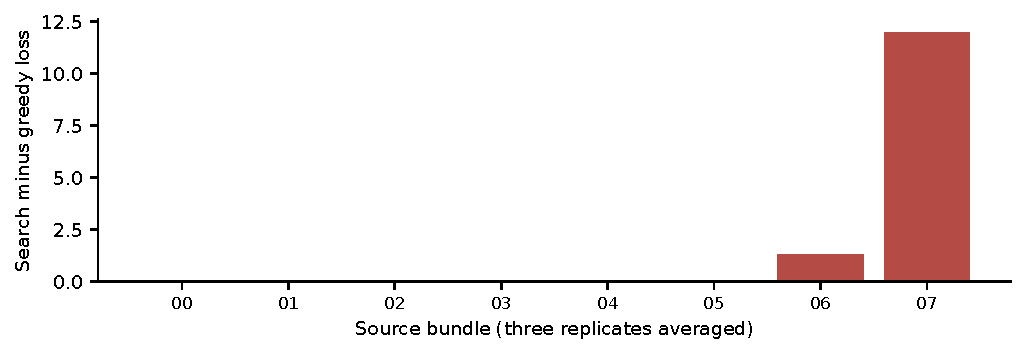
\includegraphics[width=0.98\textwidth]{../artifacts/stage6_robustness/analysis/fresh/figures/primary_bundle_differences.pdf}
\caption{All eight fresh primary bundle differences, after averaging three generation replicates. Zero values remain explicit.}
\end{figure*}
\begin{figure*}[t]
\centering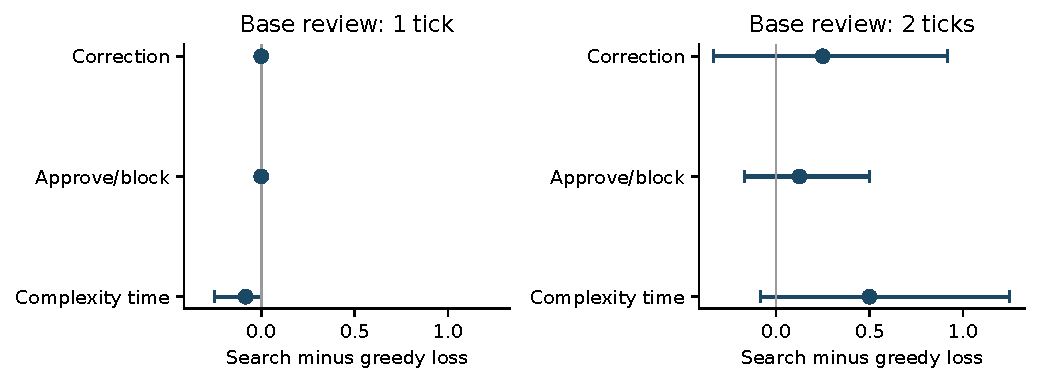
\includegraphics[width=0.98\textwidth]{../artifacts/stage6_robustness/analysis/post_hoc_stage5/figures/paired_loss.pdf}
\caption{Post hoc saved-preparation sensitivity. The 32 bundles are separate from the eight fresh bundles and are not pooled for inference.}
\end{figure*}


\section{HISTORICAL RESOURCE ACCOUNTING}
\noindent Experiments use Qwen/Qwen2.5-7B-Instruct revision
\begin{quote}\small\ttfamily
a09a35458c702b33eeacc393d103063234e8bc28
\end{quote}
on one RTX 6000 Ada, BF16, with CPU model offload and swap disabled. The reused runtime has Python 3.11.13, PyTorch 2.8.0 with CUDA 12.8, vLLM 0.10.2 and Transformers 4.55.2. The driver is 580.126.20. Driver-reported compatibility is not used as evidence of the installed runtime. CUDA BF16 computation, server arguments, model identity, process ancestry and GPU allocation are recorded together.\draftcredit

The original server on port 8000 is preserved. A separate retail server uses a 16,384-token context and 0.4 GPU-memory reservation. Requests are serial. Tokenization runs before each generation and enforces the declared input bound. Each attempt has a 60-second timeout, and each ordinary call allows one retry. Every request and failed attempt is retained in a session ledger and reconciled with raw evidence and server counters.

Earlier maintenance exact search reached six eligible requests and 1,957 ordered subsets, with 22 observed decisions averaging 4.531 ms on its recorded host. Original retail search had at most two eligible requests at actual dispatch, examining five subsets and averaging 0.05135 ms over 218 such decisions. These are bounded host-planning measurements, not a scalability guarantee or GPU latency measure.

The fresh follow-up completes 675 ordinary generation calls and 675 attempts, with zero retries, failures or unknown-token records. Requests consume 3,495,749 prompt tokens and 58,762 completion tokens. Summed HTTP generation time is 1,149.669 seconds; the preparation worker spans 1,200.660 seconds. The longest attempt lasts 4.993 seconds. Maximum observed input/output lengths are 11,369/256 tokens, within their declared limits. Server counter deltas agree exactly with the ledger and raw attempts.

There are no repeated byte-identical request groups within this fresh run. Different seeded replicates yield different proposals on eight of 24 source cases and mixed initial correctness on four. These comparisons involve different generation seeds and often later prompt histories; they do not measure identical-request nondeterminism.

Across fresh operational conditions, actual search dispatch reaches two eligible requests. Its 114 such decisions examine five ordered subsets and average 0.04832 ms, with maximum 0.11583 ms on the recorded host. Three pending requests can appear in no-review diagnostic states; the exact planner is not truncated. These repeated state measurements are descriptive.

The stage starts at 21:18:02 UTC on 10 September 2026, with inference cutoff 01:48:02 and hard deadline 03:18:02 the next day. The last generation completes at 21:57:00.893 UTC, well before the reporting reserve. The temporary server and both experimental worker processes are verified absent at 21:59:19 UTC. The original server remains healthy with unchanged counters. No new paid resources are provisioned. Provider allocation duration, price and charge are unavailable, so request time is not converted into billed cost. The final stage and cumulative clocks are reported in the repository report. Across both Stage 1 GPU demonstrations and Stages 2--6, the recorded total is 55,384 generation attempts, including two retries. No timestamp is reset to fit the original 36-hour target.

The 13,459 historical artifact, configuration and upstream files captured at authorization remain byte-identical. All 72 new GPU workflows, 864 fresh policy traces and 3,456 post hoc traces replay. The latter include 1,152 exact matches to historical retail reference traces. No fresh public evidence requires redaction; historical redaction provenance remains disclosed.


\section{EXAMPLE SELECTION}
\noindent Examples follow the frozen rule of the first numeric bundle and replicate satisfying each category under the primary restricted-authority condition. Categories are search benefit, tie, unfavorable result and preparation failure. A missing category is reported rather than filled with a convenient alternative. Full traces retain tool proposals, annotated targets for offline interpretation, review starts/completions, blocks, committed changes and incurred consequences.\draftcredit

\subsection{Fresh Unfavorable and Tied Cases}

No fresh restricted-authority run gives search lower loss than greedy. The first unfavorable run is bundle 06, replicate 2. Modification case train:466 proposes a wrong available variant. It has arrival zero, cutoff five, processing weight four and predicted error 0.2917. Cancellation case train:356 is correct, with arrival zero, cutoff two, weight twelve and predicted error 0.04. Exchange train:177 arrives at one, is correct, and has cutoff five, weight eight and predicted error 0.4762.

Search first protects the expiring cancellation, then chooses the exchange at tick two. The modification can no longer finish review after tick four and posts at five. Its service cost four plus posting cost four yields loss eight. Greedy blocks the modification at two, leaving service loss four, then approves the exchange. The unreviewed correct cancellation posts at its cutoff without error. This illustrates how preserving an opportunity under a public expected-value model can fail to preserve an actual error.

The first tie is bundle 00, replicate 0. Both policies approve the cancellation at two and block an incomplete return proposal at four. The modification has no staged proposal. Both have loss eight, consisting of the unresolved return and the unstaged modification. The first preparation failure is that modification, train:421. It finishes without a mutation; the failure field is null because no runtime exception occurs. This is still an unsuccessful retained workflow.

\subsection{Saved-Data Benefit and Failure}

The post hoc cohort contains a first qualifying benefit at bundle 28, replicate 0, with search-minus-greedy loss $-4$. Its first unfavorable case is bundle 09, replicate 0, with difference $+4$, and its first tie is bundle 00, replicate 0. The first unstaged failure is train:062 in bundle 00, replicate 2, which exhausts all 14 tool turns. The complete source intentions, proposed and annotated actions, and tick-by-tick review and posting events are saved in the companion trace files. These examples are selected by first qualification, not effect size.


\section{REPLAY AND REPRODUCTION}
\noindent From a clean checkout, saved-data analysis requires Python 3.8 or later, NumPy and Matplotlib. It makes no inference requests. The declared inference path is one-shot, deadline-guarded and separate from analysis. Reproducing a fresh model output is not guaranteed by its seed. In earlier maintenance evidence, 38 identical-request groups had mixed actions; fresh generation variation and changes in feedback-dependent prompts are separate phenomena.\draftcredit

The historical Stage 6 saved-data command, used at its recorded commit, is:
\begin{quote}\small\ttfamily
bash scripts/replay\_stage6.sh
\end{quote}
For the current measured-data package use the Stage 7 command in Section 1.4, which writes audits under Stage 7 and preserves historical evidence. The historical command verifies evidence, replays both retail cohorts, regenerates tables and builds their PDFs.
Those historical audits write under the Stage 6 root; current audits are redirected into Stage 7. Historical reference traces are checked against their original values and all historical artifact hashes are preserved. The manuscript and supplement use the unchanged official template class, style and bibliography style. Source and build details are in the reproduction guide and stage report.

Previously disclosed Stage 5 redactions remove unsolicited credential-like model text from auxiliary arguments and later prompt histories. Original request, response and file hashes remain, with exact originals retained on the authorized pod and in an ignored local evidence directory. Transactions, states, labels and accounting do not change. Public redacted prompts are not claimed to be byte-identical regeneration inputs. Any new follow-up publication redaction is separately recorded under its own evidence root.

\section*{AI ASSISTANCE}
OpenAI Codex assisted code, analysis, source checking, figure code and manuscript drafting and revision throughout this companion \cite{openai2026codex}. Reported numeric evidence comes from retained model outputs and deterministic simulation. Human authors must review and take responsibility for the complete submission. No human expert validation, author identity, funding or conflict declaration is invented.

\bibliographystyle{apalike}
{\small\bibliography{references}}
\end{document}
